\documentclass[10pt,a4paper,twocolumn]{article}

% --- PACKAGES FONDAMENTAUX ---
\usepackage[utf8]{inputenc}
\usepackage[T1]{fontenc}
\usepackage{lmodern}
\usepackage[french]{babel}
\usepackage[margin=1.65cm,top=1.8cm,bottom=1.8cm]{geometry}
\usepackage{amsmath,amssymb,amsfonts,amsthm}
\usepackage{graphicx}
\usepackage{booktabs}
\usepackage{tabularx}
\usepackage{multirow}
\usepackage{subcaption}
\usepackage{float}
\usepackage{dblfloatfix}
\usepackage{xcolor}
\usepackage{tcolorbox}
\usepackage{cite}
\usepackage{placeins}
\usepackage[expansion=false]{microtype}
\usepackage{titlesec}
\usepackage{fancyhdr}
\usepackage{hyperref}

% --- COULEURS ET CHARTE GRAPHIQUE ---
\definecolor{inseaBlue}{RGB}{20, 55, 90}
\definecolor{inseaGold}{RGB}{185, 140, 40}
\definecolor{darkgreen}{RGB}{20, 110, 50}
\definecolor{darkred}{RGB}{160, 25, 25}
\definecolor{boxbg}{RGB}{245, 248, 252}

\hypersetup{
    colorlinks=true,
    linkcolor=inseaBlue,
    citecolor=inseaBlue,
    urlcolor=inseaBlue,
    pdftitle={Rapport Machine Learning - Reconnaissance Varietes Haricots Secs},
    pdfauthor={Equipe ML INSEA}
}

% --- EN-TETES ET PIEDS DE PAGE ---
\pagestyle{fancy}
\fancyhf{}
\fancyhead[L]{\small\color{gray}INSEA 2026--2027 | Module de Machine Learning}
\fancyhead[R]{\small\color{gray}Mini-Projet 02 : Classification UCI Dry Bean}
\fancyfoot[C]{\thepage}
\renewcommand{\headrulewidth}{0.4pt}

% --- SECTIONS POLISSAGE ---
\titleformat{\section}{\color{inseaBlue}\normalfont\large\bfseries}{\thesection.}{0.5em}{}[\titlerule]
\titleformat{\subsection}{\color{inseaBlue}\normalfont\normalsize\bfseries}{\thesubsection.}{0.4em}{}
\titleformat{\subsubsection}{\color{black}\normalfont\small\bfseries}{\thesubsubsection.}{0.3em}{}

% --- GESTION DES FLOTTANTS (PAGES COMPACTES) ---
\renewcommand{\topfraction}{0.95}
\renewcommand{\bottomfraction}{0.95}
\renewcommand{\textfraction}{0.05}
\renewcommand{\floatpagefraction}{0.85}
\renewcommand{\dbltopfraction}{0.95}
\renewcommand{\dblfloatpagefraction}{0.85}

% --- BOITE PROTOCOLE ---
\newtcolorbox{protocolbox}[1]{
    colback=boxbg,
    colframe=inseaBlue,
    fonttitle=\bfseries\small,
    title=#1,
    arc=1.5mm,
    boxrule=0.7pt,
    left=2mm, right=2mm, top=1.5mm, bottom=1.5mm
}

% --- TITRE DU DOCUMENT ---
\title{
    \vspace{-2.8cm}
    \includegraphics[height=3cm]{figures/logo.png}\\[0.01cm]


    
    \small\textbf{INSTITUT NATIONAL DE STATISTIQUE ET D'ÉCONOMIE APPLIQUÉE}\\[0.15cm]
    \LARGE\textbf{\color{inseaBlue}Reconnaissance Automatisée de Variétés de Haricots Secs par Apprentissage Supervisé}\\[0.2cm]
    \large\textit{Étude Comparative et Benchmark de Cinq Architectures sur le Dataset UCI Dry Bean}
}

\author{
    \textbf{Équipe :}\\
    \textbf{Youssef FATIMI} (DSE) \quad 
    \textbf{Hamza BALLA} (DSE) \\
    \textbf{Mohamed Yahya SAFADI} (DSE) \quad 
    \textbf{Ayoub ELHANAFI} (DSE) \\[0.25cm]
    \small \textit{Sous la direction académique de :} \textbf{Pr. Saidi}
}
\date{Année Universitaire : 2026-2027}

\begin{document}

\twocolumn[
  \begin{@twocolumnfalse}
    \maketitle
    \begin{abstract}
    \noindent Ce travail répond au cahier des charges du Mini-Projet 02 du cours de Machine Learning. À partir de 16 caractéristiques morphologiques extraites d'images de 13\,611 grains de haricots secs (\textit{UCI Dry Bean Dataset}), nous développons, optimisons et comparons cinq familles de classifieurs supervisés pour reconnaître sept variétés commerciales (\textit{Barbunya, Bombay, Cali, Dermason, Horoz, Seker, Sira}) sans traiter directement les images. Conformément au protocole imposé, l'évaluation repose sur un découpage stratifié étanche (80\,\% Train / 20\,\% Test, $\texttt{SEED}=42$) et une validation croisée stratifiée à 5 plis au sein de \texttt{Pipelines} Scikit-Learn pour prévenir toute fuite d'information (\textit{Zero Data Leakage}). Face au déséquilibre des classes (de 3.84\,\% pour Bombay à 26.05\,\% pour Dermason), le \textbf{F1-score Macro} est la métrique cardinale d'évaluation. Une étude d'ablation démontre l'impact décisif du centrage-réduction pour les modèles métriques et à gradients (+33.60 points pour le SVM, +22.17 pour KNN) et son invariance stricte sur les arbres (0.00 point). Sur le jeu de test scellé (2\,723 grains), le \textbf{SVM à noyau RBF} ($C=5, \gamma=0.1$) s'impose comme champion avec un \textbf{F1-score Macro de 0.9363} et une \textbf{Accuracy de 92.47\,\%}. Enfin, la dissection de la matrice de confusion $7 \times 7$ met en lumière les confusions majeures du problème, notamment entre Dermason et Sira (46.8\,\% des erreurs totales).
    \end{abstract}
    \vspace{0.35cm}
  \end{@twocolumnfalse}
]

% ==============================================================================
\section{Contexte \& Problématique}
\label{sec:intro}
% ==============================================================================

Le calibrage et le contrôle de pureté variétale des légumineuses représentent un enjeu agronomique majeur~\cite{koklu2020multiclass}. Chez le haricot sec (\textit{Phaseolus vulgaris L.}), mélanger involontairement des variétés distinctes altère l'homogénéité de cuisson et déprécie la valeur marchande du lot. Traditionnellement manuel et fastidieux, ce tri gagne à être automatisé par vision artificielle et apprentissage automatique.

L'objectif de ce mini-projet est de développer et de comparer plusieurs classifieurs capables de distinguer sept variétés de haricots secs à partir de 16 caractéristiques morphologiques pré-extraites, \textbf{sans traiter directement les images}.

La question centrale posée par le cahier des charges est la suivante : \textit{Quels modèles distinguent le mieux les sept variétés et quelles classes restent les plus difficiles à reconnaître ?}

Pour y répondre, nous comparons cinq architectures de référence :
\begin{enumerate}
    \item La \textbf{Régression Logistique Multiclasse} (Softmax) ;
    \item Les \textbf{K-Plus Proches Voisins} (KNN) ;
    \item L'\textbf{Arbre de Décision} (CART) ;
    \item La \textbf{Forêt Aléatoire} (\textit{Random Forest}) ;
    \item Les \textbf{Machines à Vecteurs de Support} (SVM).
\end{enumerate}

% ==============================================================================
\section{Données \& Exploration Graphique}
\label{sec:eda}
% ==============================================================================

\subsection{Description du Corpus UCI Dry Bean}
Le jeu de données officiel \textit{UCI Dry Bean Dataset}~\cite{koklu2020multiclass} comprend $N = 13\,611$ observations individuelles sans aucune valeur manquante. Chaque grain est décrit par 16 variables continues :
\begin{itemize}
    \item \textbf{12 Caractéristiques Géométriques :} \texttt{Area}, \texttt{Perimeter}, \texttt{MajorAxisLength}, \texttt{MinorAxisLength}, \texttt{AspectRation}, \texttt{Eccentricity}, \texttt{ConvexArea}, \texttt{EquivDiameter}, \texttt{Extent}, \texttt{Solidity}, \texttt{roundness}, \texttt{Compactness}.
    \item \textbf{4 Facteurs de Forme :} \texttt{ShapeFactor1} à \texttt{ShapeFactor4}, sans dimension et invariants à l'échelle.
\end{itemize}

\begin{table}[h]
\centering
\small
\caption{Répartition des sept variétés dans le corpus}
\label{tab:classes}
\begin{tabular}{@{}llcc@{}}
\toprule
\textbf{Variété} & \textbf{Code / Label} & \textbf{Effectif} & \textbf{Proportion} \\
\midrule
Dermason & \texttt{DERMASON} & 3\,546 & 26.05\,\% \\
Sira     & \texttt{SIRA}     & 2\,636 & 19.37\,\% \\
Seker    & \texttt{SEKER}    & 2\,027 & 14.89\,\% \\
Horoz    & \texttt{HOROZ}    & 1\,928 & 14.16\,\% \\
Cali     & \texttt{CALI}     & 1\,630 & 11.98\,\% \\
Barbunya & \texttt{BARBUNYA} & 1\,322 & 9.71\,\% \\
Bombay   & \texttt{BOMBAY}   & 522   & 3.84\,\% \\
\midrule
\textbf{Total} & \textbf{7 classes} & \textbf{13\,611} & \textbf{100.00\,\%} \\
\bottomrule
\end{tabular}
\end{table}

\begin{figure}[h]
\centering
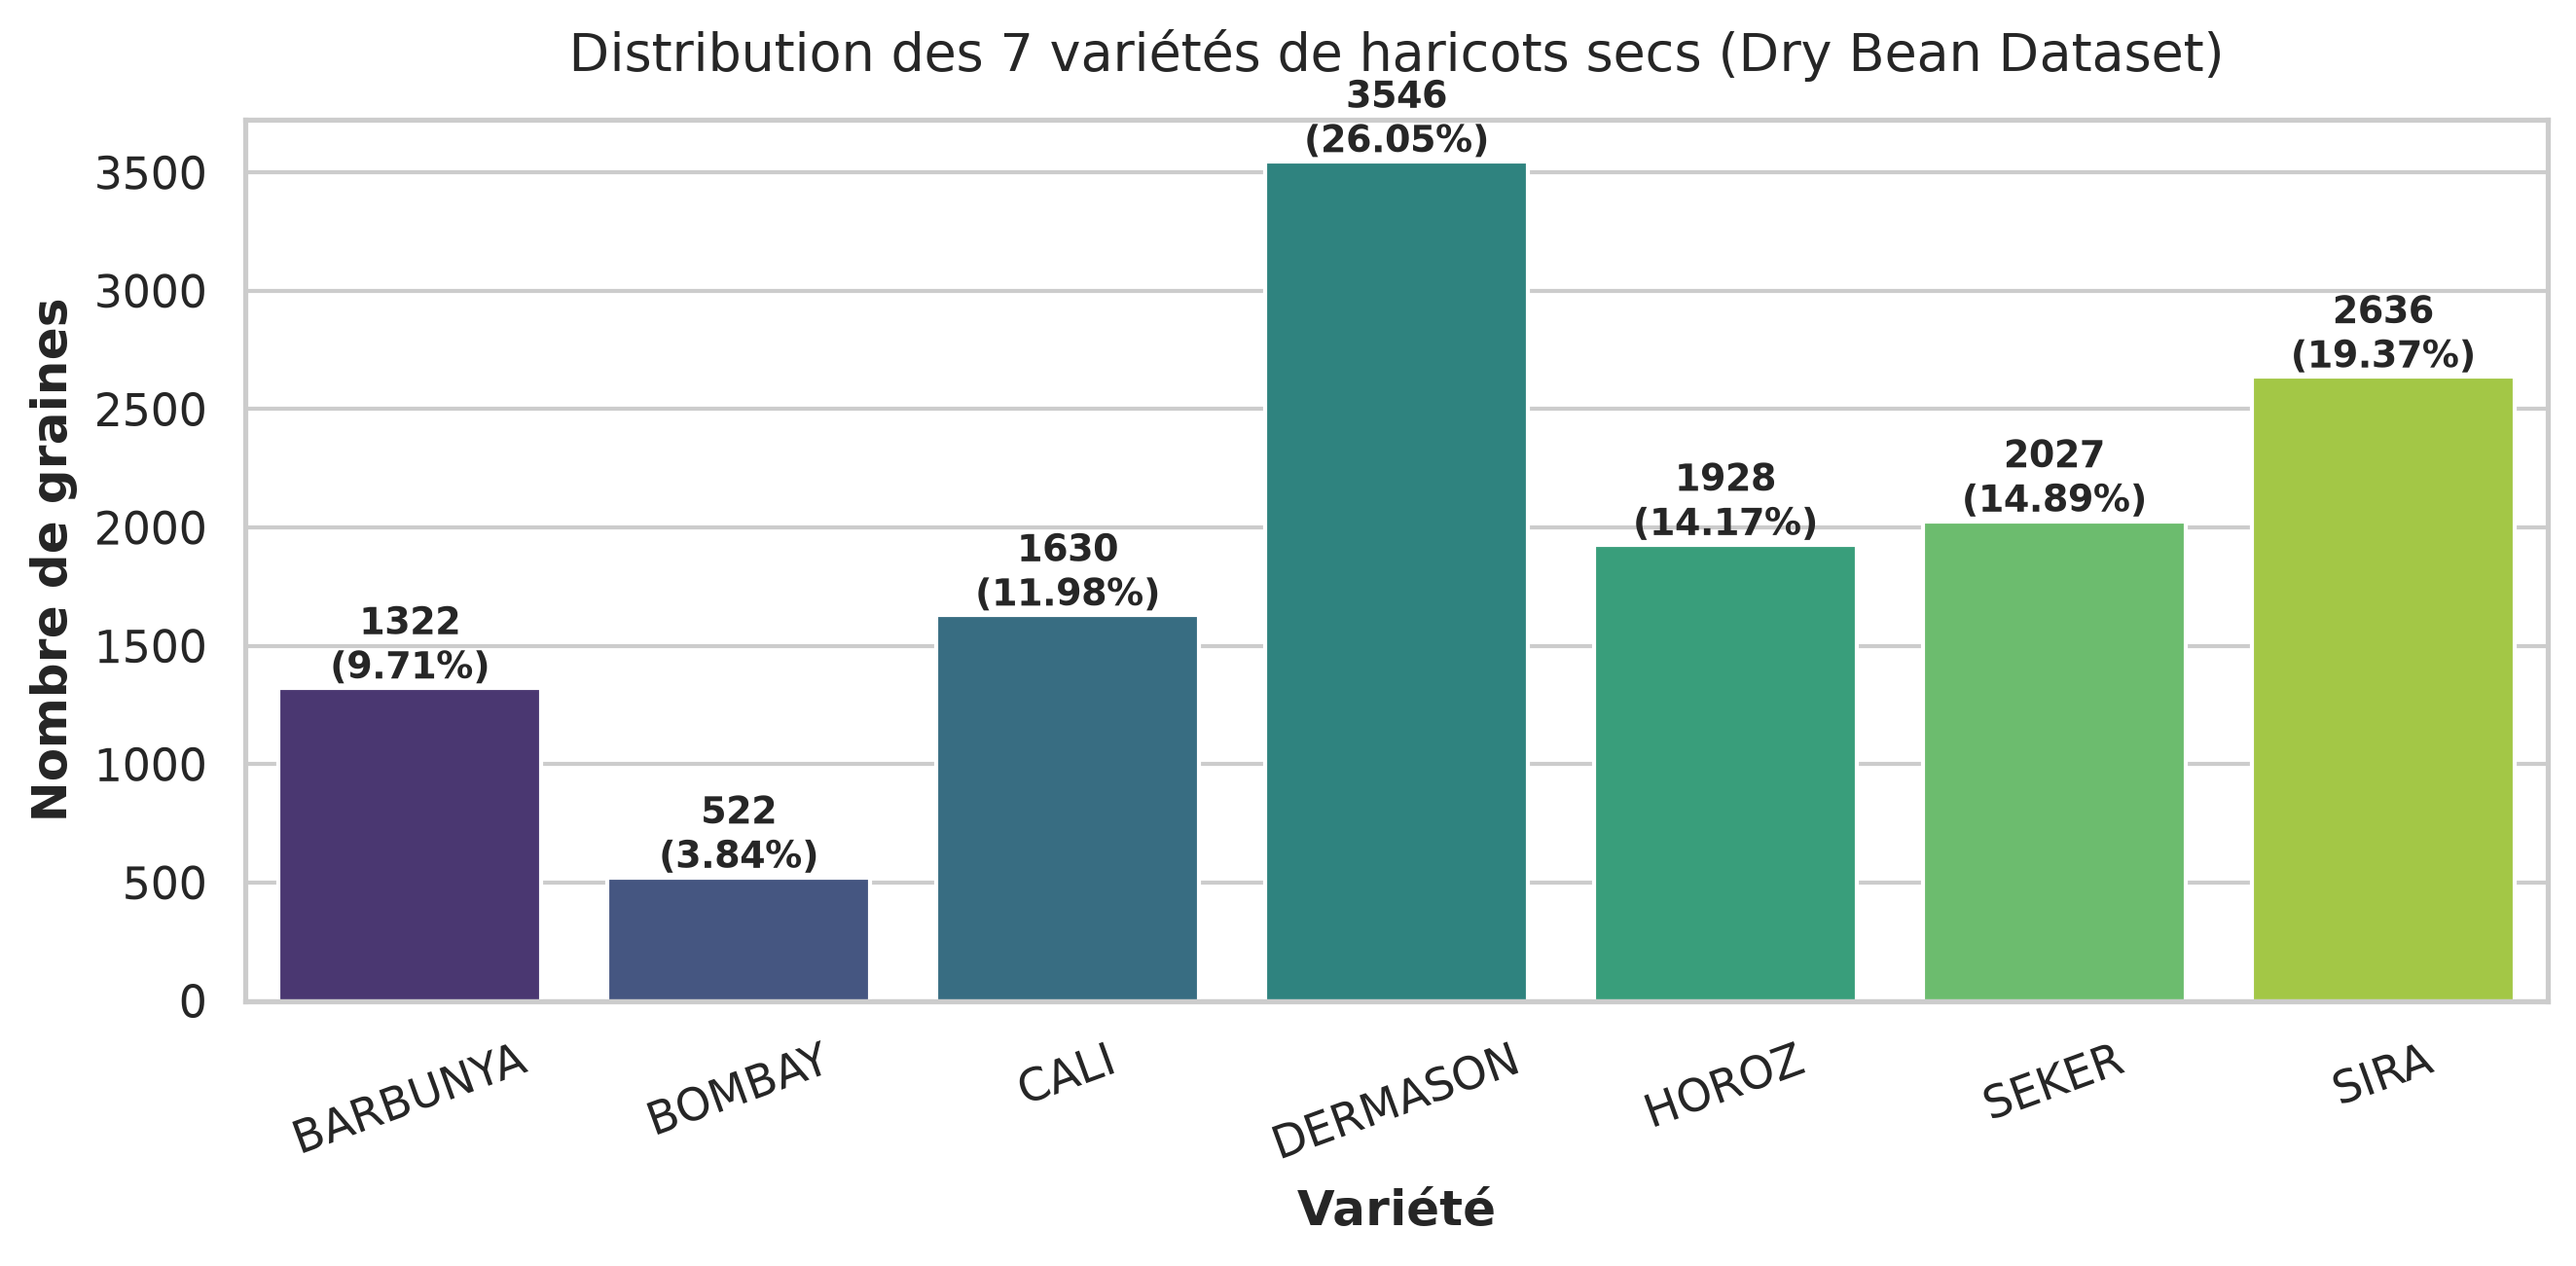
\includegraphics[width=\columnwidth]{figures/01_eda_classes_distribution.png}
\caption{Distribution des effectifs par variété de haricot sec.}
\label{fig:eda_dist}
\end{figure}

\subsection{Déséquilibre de Classes \& Métrique d'Arbitrage}
Le Tableau~\ref{tab:classes} et la Figure~\ref{fig:eda_dist} révèlent une forte asymétrie d'effectifs : \texttt{DERMASON} regroupe plus du quart du corpus (26.05\,\%) tandis que \texttt{BOMBAY} n'en représente que 3.84\,\%, soit un ratio de 1 à 6.8.

L'exactitude brute (\textit{Accuracy}) est donc trompeuse : un modèle prédisant systématiquement les classes majoritaires obtiendrait une note élevée tout en ignorant les variétés rares. Conformément aux consignes, nous privilégions le \textbf{F1-score Macro}, moyenne arithmétique non pondérée des scores harmoniques de chaque classe $k \in \{1, \dots, K\}$ :
\begin{equation}
F_{1, \text{macro}} = \frac{1}{K} \sum_{k=1}^K F_{1, k} = \frac{1}{K} \sum_{k=1}^K \frac{2 \cdot P_k \cdot R_k}{P_k + R_k}
\label{eq:f1_macro}
\end{equation}

\begin{figure*}[t]
\centering
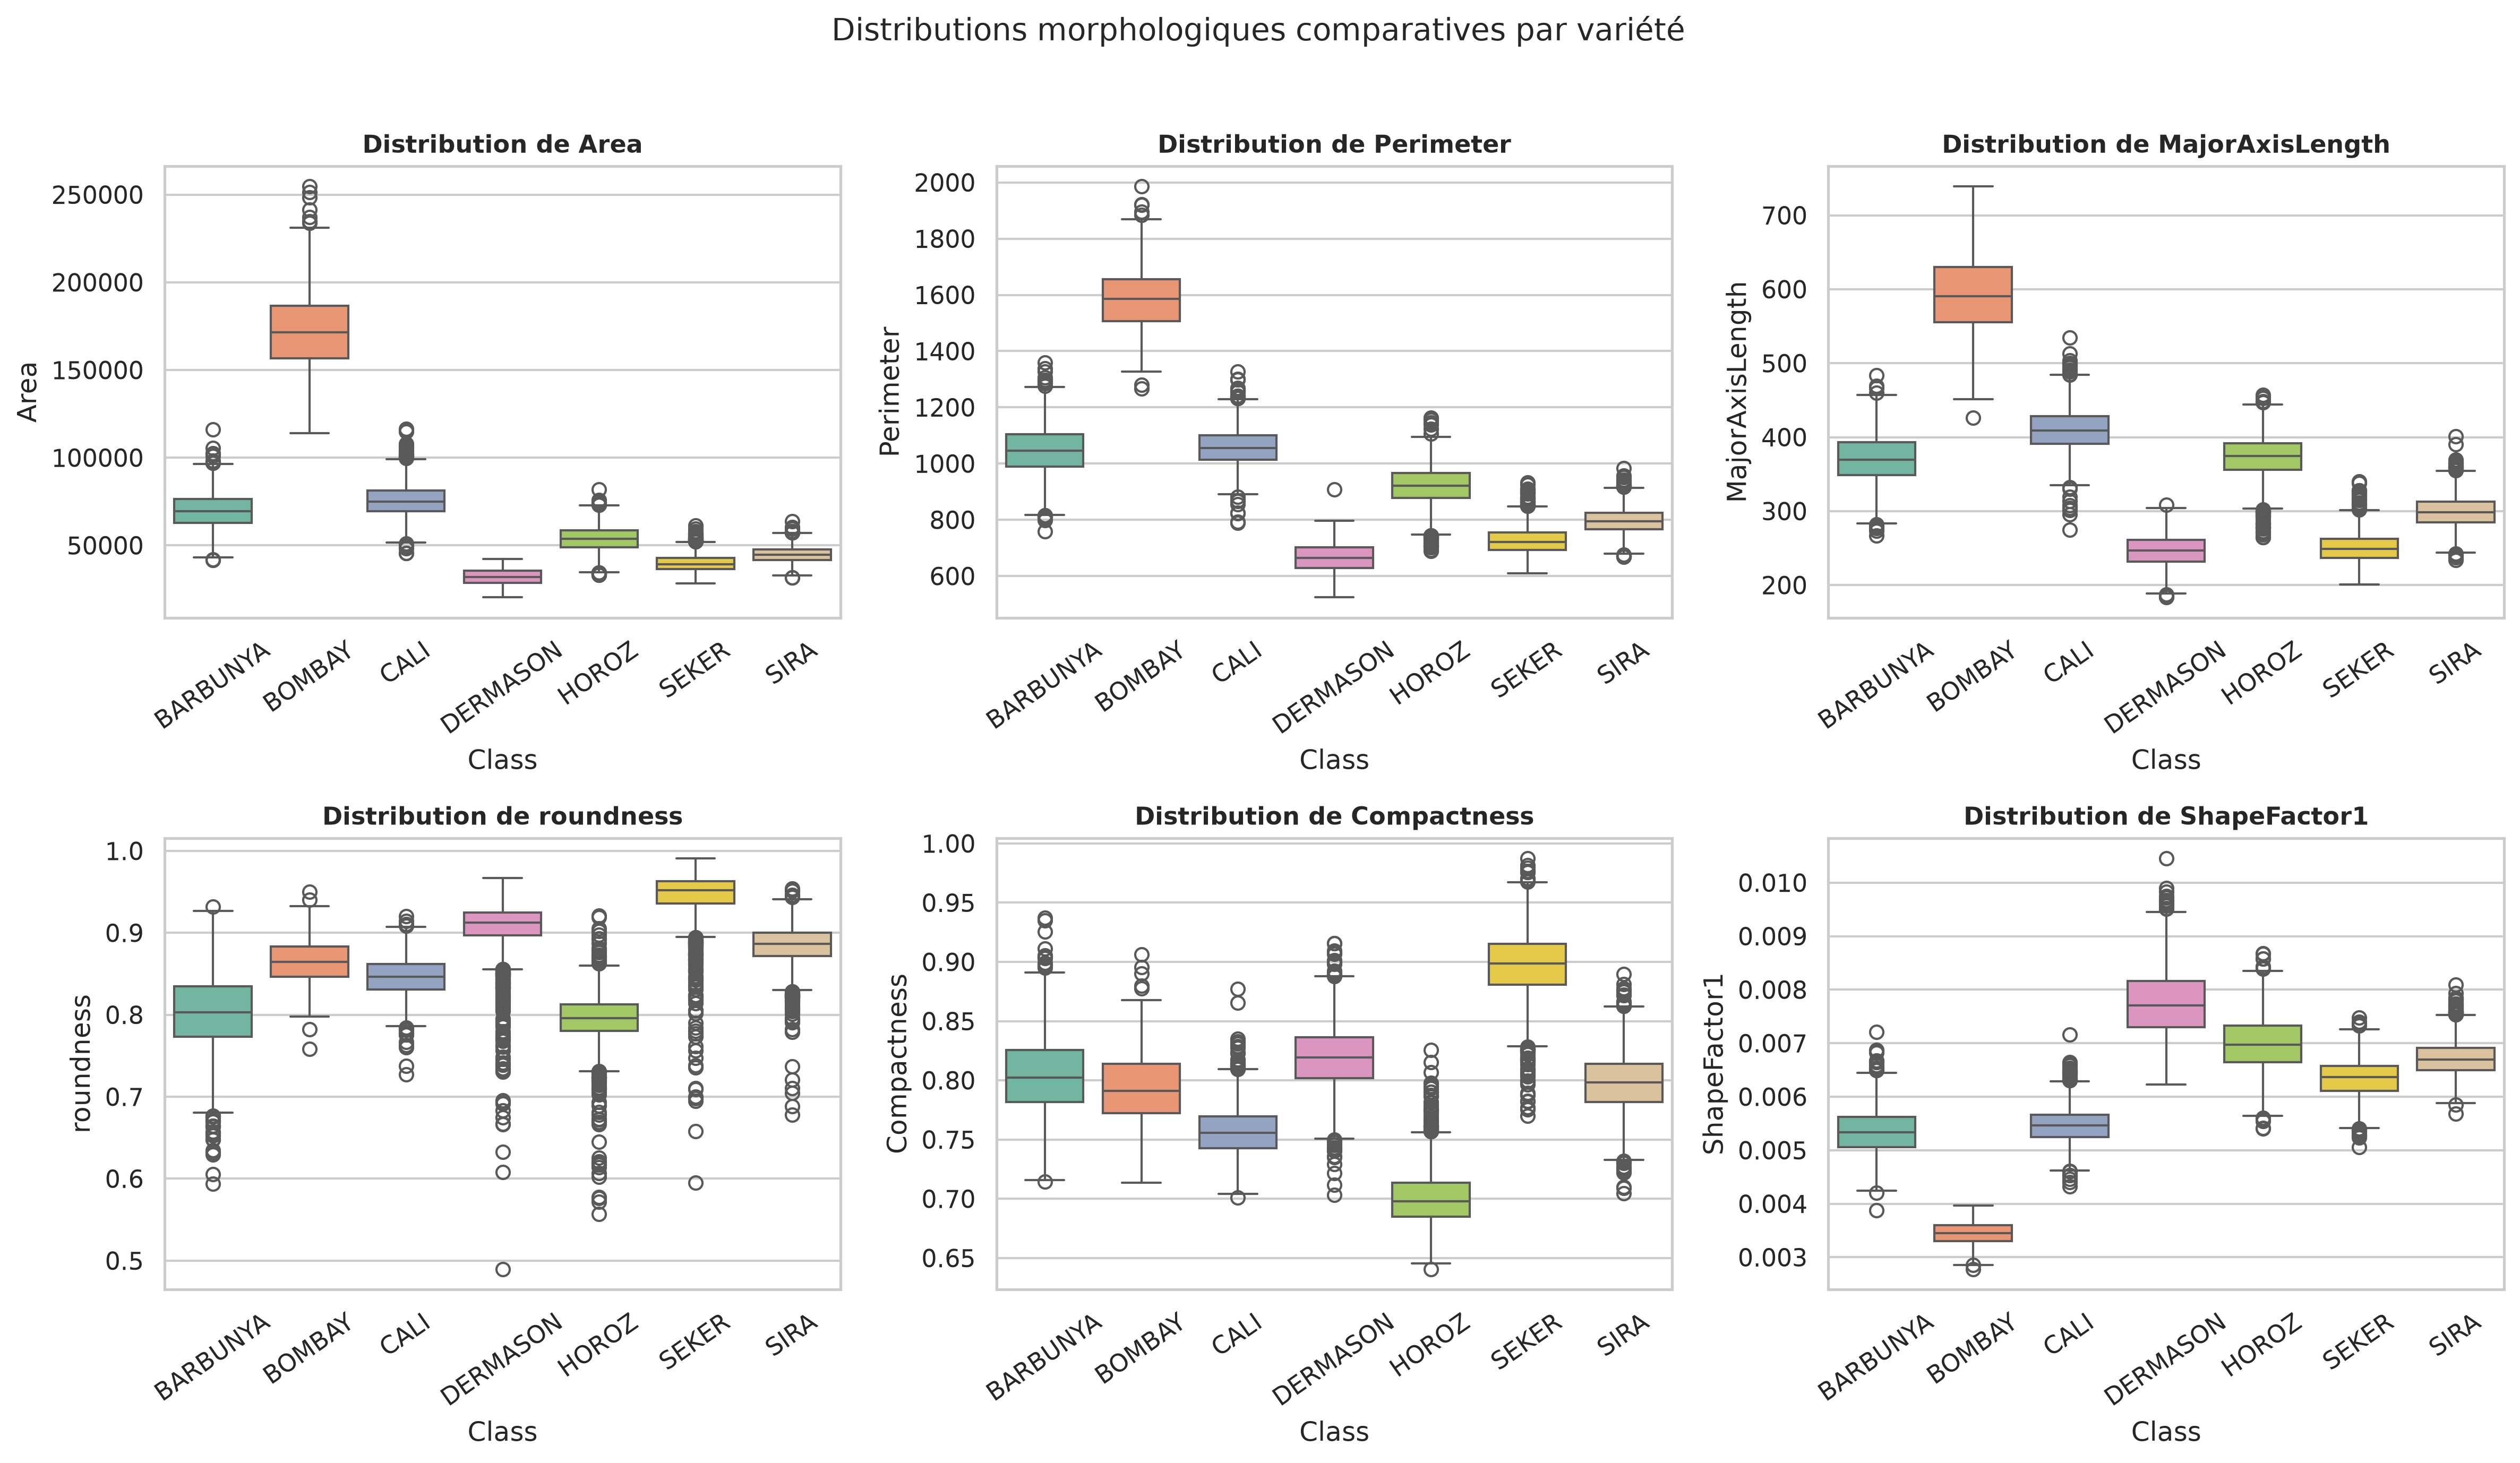
\includegraphics[width=0.88\textwidth,height=4.6cm,keepaspectratio]{figures/02_eda_morphological_boxplots.png}
\caption{Distributions comparatives des principaux descripteurs morphologiques par variété de haricot.}
\label{fig:eda_boxplots}
\end{figure*}

\subsection{Distributions Morphologiques \& Invariants}
L'examen des boîtes à moustaches (Figure~\ref{fig:eda_boxplots}) dégage les invariants physiques du corpus :
\begin{enumerate}
    \item \textbf{Bombay (Géant) :} Aire médiane $\approx 173\,000$ px² contre moins de $70\,000$ px² pour les autres variétés. Séparabilité quasi linéaire immédiate.
    \item \textbf{Horoz (Allongé) :} Ratio d'aspect et excentricité maximaux, traduisant une forme cylindrique allongée.
    \item \textbf{Seker (Sphérique) :} Circularité et compacité maximales ($\approx 0.94$).
    \item \textbf{Dermason / Sira (Piège morphologique) :} Distributions d'aire, de périmètre et de compacité presque superposées. C'est le foyer d'erreur majeur attendu.
\end{enumerate}
Par ailleurs, les descripteurs de taille (\texttt{Area}, \texttt{Perimeter}, \texttt{ConvexArea}) présentent des corrélations de Pearson quasi unitaires ($r \ge 0.98$), imposant une régularisation ($L_2$) sur les modèles paramétriques.

% ==============================================================================
\section{Protocole Expérimental \& Ablation}
\label{sec:protocol}
% ==============================================================================

\subsection{Protocole Expérimental Obligatoire}
Afin de garantir une comparabilité sans biais, l'équipe applique un protocole unifié respectant scrupuleusement les exigences du cours :

\begin{protocolbox}{Protocole Expérimental Commun (Règle d'Or)}
\begin{itemize}\setlength{\itemsep}{1.5pt}\setlength{\parskip}{0pt}\small
    \item \textbf{Graine Aléatoire Universelle :} $\texttt{SEED} = 42$ commune.
    \item \textbf{Partitionnement Étanche :} 80\,\% Train ($N = 10\,888$) / 20\,\% Test ($N = 2\,723$), avec stratification stricte sur la variété cible.
    \item \textbf{Zero Data Leakage :} Le centrage-réduction (\texttt{StandardScaler}) est appris (\texttt{fit}) exclusivement sur les plis d'entraînement internes via l'encapsulation dans un \texttt{Pipeline} Scikit-Learn~\cite{pedregosa2011scikit}.
    \item \textbf{Validation Croisée Stratifiée :} $K=5$ plis (\texttt{StratifiedKFold}) sur le train set pour toutes les grilles de réglage (\texttt{GridSearchCV}).
    \item \textbf{Isolation du Test Set :} Évalué une seule fois à la fin.
\end{itemize}
\end{protocolbox}

\begin{table}[h]
\centering
\small
\caption{Vérification de la stratification Train / Test}
\label{tab:strat}
\begin{tabular}{@{}lccc@{}}
\toprule
\textbf{Variété} & \textbf{Corpus (\%)} & \textbf{Train (\%)} & \textbf{Test (\%)} \\
\midrule
Dermason & 26.05\,\% & 26.05\,\% & 26.04\,\% \\
Sira     & 19.37\,\% & 19.37\,\% & 19.35\,\% \\
Seker    & 14.89\,\% & 14.89\,\% & 14.91\,\% \\
Horoz    & 14.16\,\% & 14.16\,\% & 14.18\,\% \\
Cali     & 11.98\,\% & 11.98\,\% & 11.97\,\% \\
Barbunya & 9.71\,\%  & 9.71\,\%  & 9.70\,\% \\
Bombay   & 3.84\,\%  & 3.84\,\%  & 3.86\,\% \\
\bottomrule
\end{tabular}
\end{table}

Le Tableau~\ref{tab:strat} démontre que la stratification préserve exactement les fréquences marginales au centième de pourcent près.

\subsection{Expérience d'Ablation : Impact du Centrage-Réduction}
L'écart d'échelle entre \texttt{Area} ($\approx 10^5$) et \texttt{ShapeFactor1} ($\approx 10^{-3}$) constitue un piège classique. Nous avons mené une étude d'ablation systématique par CV 5-plis sur l'entraînement, comparant les cinq algorithmes avec et sans standardisation Z-score ($z = \frac{x-\mu}{\sigma}$).

\begin{table}[h]
\centering
\small
\caption{Résultats de l'expérience d'ablation sur la standardisation}
\label{tab:ablation}
\resizebox{\columnwidth}{!}{
\begin{tabular}{@{}lccc@{}}
\toprule
\textbf{Algorithme} & \textbf{Sans Scaling} & \textbf{Avec Scaling} & \textbf{Gain (pts)} \\
\midrule
\textbf{SVM (Noyau RBF)} & 0.5983 & \textbf{0.9343} & \textbf{+33.60} \\
\textbf{KNN ($k=9$)}      & 0.7138 & \textbf{0.9355} & \textbf{+22.17} \\
\textbf{Régression Log.} & 0.7544 & \textbf{0.9329} & \textbf{+17.85} \\
\textbf{Forêt Aléatoire} & 0.9321 & 0.9321 & \textbf{0.00} \\
\textbf{Arbre CART}      & 0.9194 & 0.9194 & \textbf{0.00} \\
\bottomrule
\end{tabular}
}
\end{table}

Les résultats du Tableau~\ref{tab:ablation} confirment les enseignements théoriques du cours :
\begin{itemize}
    \item \textbf{Modèles Métriques et à Gradients (Sensibilité Critique) :} Sans mise à l'échelle, la distance euclidienne dans KNN et le noyau gaussien dans SVM $\exp(-\gamma \|x_i - x_j\|^2)$ sont écrasés par la variable \texttt{Area}, causant une chute spectaculaire de \textbf{-33.60 points de F1} pour SVM et \textbf{-22.17 points} pour KNN.
    \item \textbf{Modèles Arborescents (Invariance Stricte) :} Les critères de division de CART et Random Forest reposent uniquement sur l'ordre des valeurs ($x_j \le s$). Toute transformation monotone strictement croissante préserve l'ordre, expliquant le gain strictement nul (\textbf{0.00 point}).
\end{itemize}

% ==============================================================================
\section{Modélisation \& Optimisation des Modèles}
\label{sec:models}
% ==============================================================================

Conformément aux exigences du cahier des charges, chaque algorithme a fait l'objet d'une recherche d'hyperparamètres rigoureuse par validation croisée stratifiée à 5 plis (\texttt{GridSearchCV}) sur les données d'entraînement ($N_{\text{train}} = 10\,888$), en retenant le F1-score macro comme critère d'arbitrage.

\subsection{Modèle 1 -- Régression Logistique Multiclasse}
La régression logistique multinomiale modélise la probabilité a posteriori de chaque variété par la fonction Softmax~\cite{bishop2006pattern} associée à une régularisation de Tikhonov ($L_2$) :
\begin{equation}
P(y = k \mid \mathbf{x}) = \frac{\exp(\mathbf{w}_k^T \mathbf{x} + b_k)}{\sum_{j=1}^7 \exp(\mathbf{w}_j^T \mathbf{x} + b_j)}
\label{eq:softmax}
\end{equation}
L'optimisation conjointe par l'algorithme quasi-Newton L-BFGS sur la grille de pénalité $C \in \{0.01, 0.1, 1, 10, 100\}$ sélectionne $C^* = 100$. Ce paramètre de régularisation modéré démontre que la standardisation préalable conditionne idéalement la matrice hessienne du problème convexe, assurant une convergence numérique rapide sans risque de sur-apprentissage.

\subsection{Modèle 2 -- K-Plus Proches Voisins (KNN)}
Classifieur géométrique non paramétrique estimant la densité locale par vote de voisinage~\cite{cover1967nearest}. La grille de recherche a exploré conjointement le nombre de voisins $k \in \{1, 3, 5, \dots, 41\}$, les métriques de Minkowski ($L_1$, $L_2$, $L_\infty$) et la règle d'agrégation (\texttt{uniform} vs \texttt{distance}). La configuration optimale retenue est :
\begin{equation}
\theta^*_{\text{KNN}} = \{k^* = 9, \quad \text{distance euclidienne } L_2, \quad w_i = 1/d\}
\end{equation}
La pondération par l'inverse de la distance ($w_i = 1/d$) apporte un gain décisif par rapport à la règle uniforme : elle atténue l'effet de flou dans les régions frontalières denses en accordant un poids prépondérant aux plus proches voisins immédiats. Les valeurs extrêmes ($k \le 3$) provoquent un sur-ajustement aux artefacts locaux, tandis que les grands voisinages ($k \ge 31$) écrasent les petites classes.

\subsection{Modèle 3 -- Arbre de Décision CART}
L'arbre de classification binaire partitionne récursivement l'espace des caractéristiques en minimisant l'impureté de Gini à chaque coupure : $I_G(t) = 1 - \sum_{k=1}^7 p_{k|t}^2$~\cite{breiman2001random}. L'analyse de la courbe de complexité sur $\texttt{max\_depth} \in \{3, \dots, 20\}$ désigne $\texttt{max\_depth}^* = 9$ comme le compromis optimal. Un arbre non élagué ($\texttt{max\_depth} \ge 15$) apprend par cœur les micro-variations de l'échantillon d'apprentissage ($F_{1,\text{train}} \approx 0.99$ mais décrochage en généralisation), tandis que $\texttt{max\_depth}^* = 9$ stabilise les séparations.

\subsection{Modèle 4 -- Forêt Aléatoire (Random Forest)}
Ensemble de $B = 200$ arbres CART décorrélés par double stochasticité (\textit{bagging} d'observations et sélection aléatoire de $\sqrt{p} = \sqrt{16} = 4$ variables candidates par nœud)~\cite{breiman2001random}. La grille a croisé $n \in \{100, 200, 300\}$ estimateurs et $\texttt{max\_depth} \in \{10, 15, 20\}$. La combinaison optimale retient $n^* = 200$ et $\texttt{max\_depth}^* = 15$. L'agrégation par vote majoritaire réduit drastiquement la variance de l'estimateur sans altérer son biais, procurant un gain net de +1.27 point de F1 macro face à l'arbre CART individuel.

\subsection{Modèle 5 -- Support Vector Machines (SVM)}
Recherche de l'hyperplan optimal maximisant la marge géométrique avec variables d'écart souples $\xi_i \ge 0$ pour gérer les recouvrements partiels de distributions~\cite{cortes1995support} :
\begin{equation}
\min_{\mathbf{w}, b, \boldsymbol{\xi}} \frac{1}{2} \|\mathbf{w}\|^2 + C \sum_{i=1}^N \xi_i \quad \text{s.t.} \quad y_i(\mathbf{w}^T \phi(\mathbf{x}_i) + b) \ge 1 - \xi_i
\label{eq:svm_primal}
\end{equation}
Nous avons confronté le SVM linéaire et le SVM à noyau à base de fonctions radiales (RBF) $K(\mathbf{x}_i, \mathbf{x}_j) = \exp(-\gamma \|\mathbf{x}_i - \mathbf{x}_j\|^2)$. L'optimisation conjointe sur grille fine $\{C \in [0.1, 100], \gamma \in [0.001, 1]\}$ retient :
\begin{equation}
\theta^*_{\text{SVM}} = \{C^* = 5, \quad \gamma^* = 0.1\}
\end{equation}
Le noyau RBF projette les descripteurs dans un espace hilbertien de dimension infinie, surclassant nettement le noyau linéaire ($F_1 = 0.9302$) de +0.61 point grâce à sa flexibilité face aux frontières de décision hautement non linéaires.

% Flottants pour Page 4 déclarés ici
\begin{table*}[t]
\centering
\small
\caption{Grand Benchmark Comparatif des 5 architectures sur le jeu de test indépendant ($N_{\text{test}} = 2\,723$)}
\label{tab:benchmark}
\resizebox{\textwidth}{!}{
\begin{tabular}{@{}llcccccr@{}}
\toprule
\textbf{Rang / Modèle} & \textbf{Hyperparamètres Optimaux} & \textbf{F1 CV (Train)} & \textbf{Accuracy (\%)} & \textbf{Précision} & \textbf{Rappel} & \textbf{F1 Macro} & \textbf{Inférence (ms)} \\
\midrule
1. \textbf{SVM (Noyau RBF)} & $C=5, \gamma=0.1$ & \textbf{0.9388} & \textbf{92.47\,\%} & \textbf{0.9366} & \textbf{0.9362} & \textbf{0.9363} & 15.2 ms \\
2. \textbf{Régression Logistique} & $C=100$ & 0.9329 & 92.10\,\% & 0.9333 & 0.9327 & 0.9329 & \textbf{2.1 ms} \\
3. \textbf{Random Forest} & $n=200, \texttt{depth}=15$ & 0.9365 & 92.25\,\% & 0.9325 & 0.9320 & 0.9321 & 28.4 ms \\
4. \textbf{KNN (Pondéré)} & $k=9, \text{euclidien, distance}$ & 0.9382 & 92.18\,\% & 0.9304 & 0.9298 & 0.9300 & 45.1 ms \\
5. \textbf{Arbre CART} & $\texttt{max\_depth}=9$ & 0.9194 & 90.56\,\% & 0.9196 & 0.9193 & 0.9194 & 0.9 ms \\
\bottomrule
\end{tabular}
}
\end{table*}

\begin{figure*}[t]
\centering
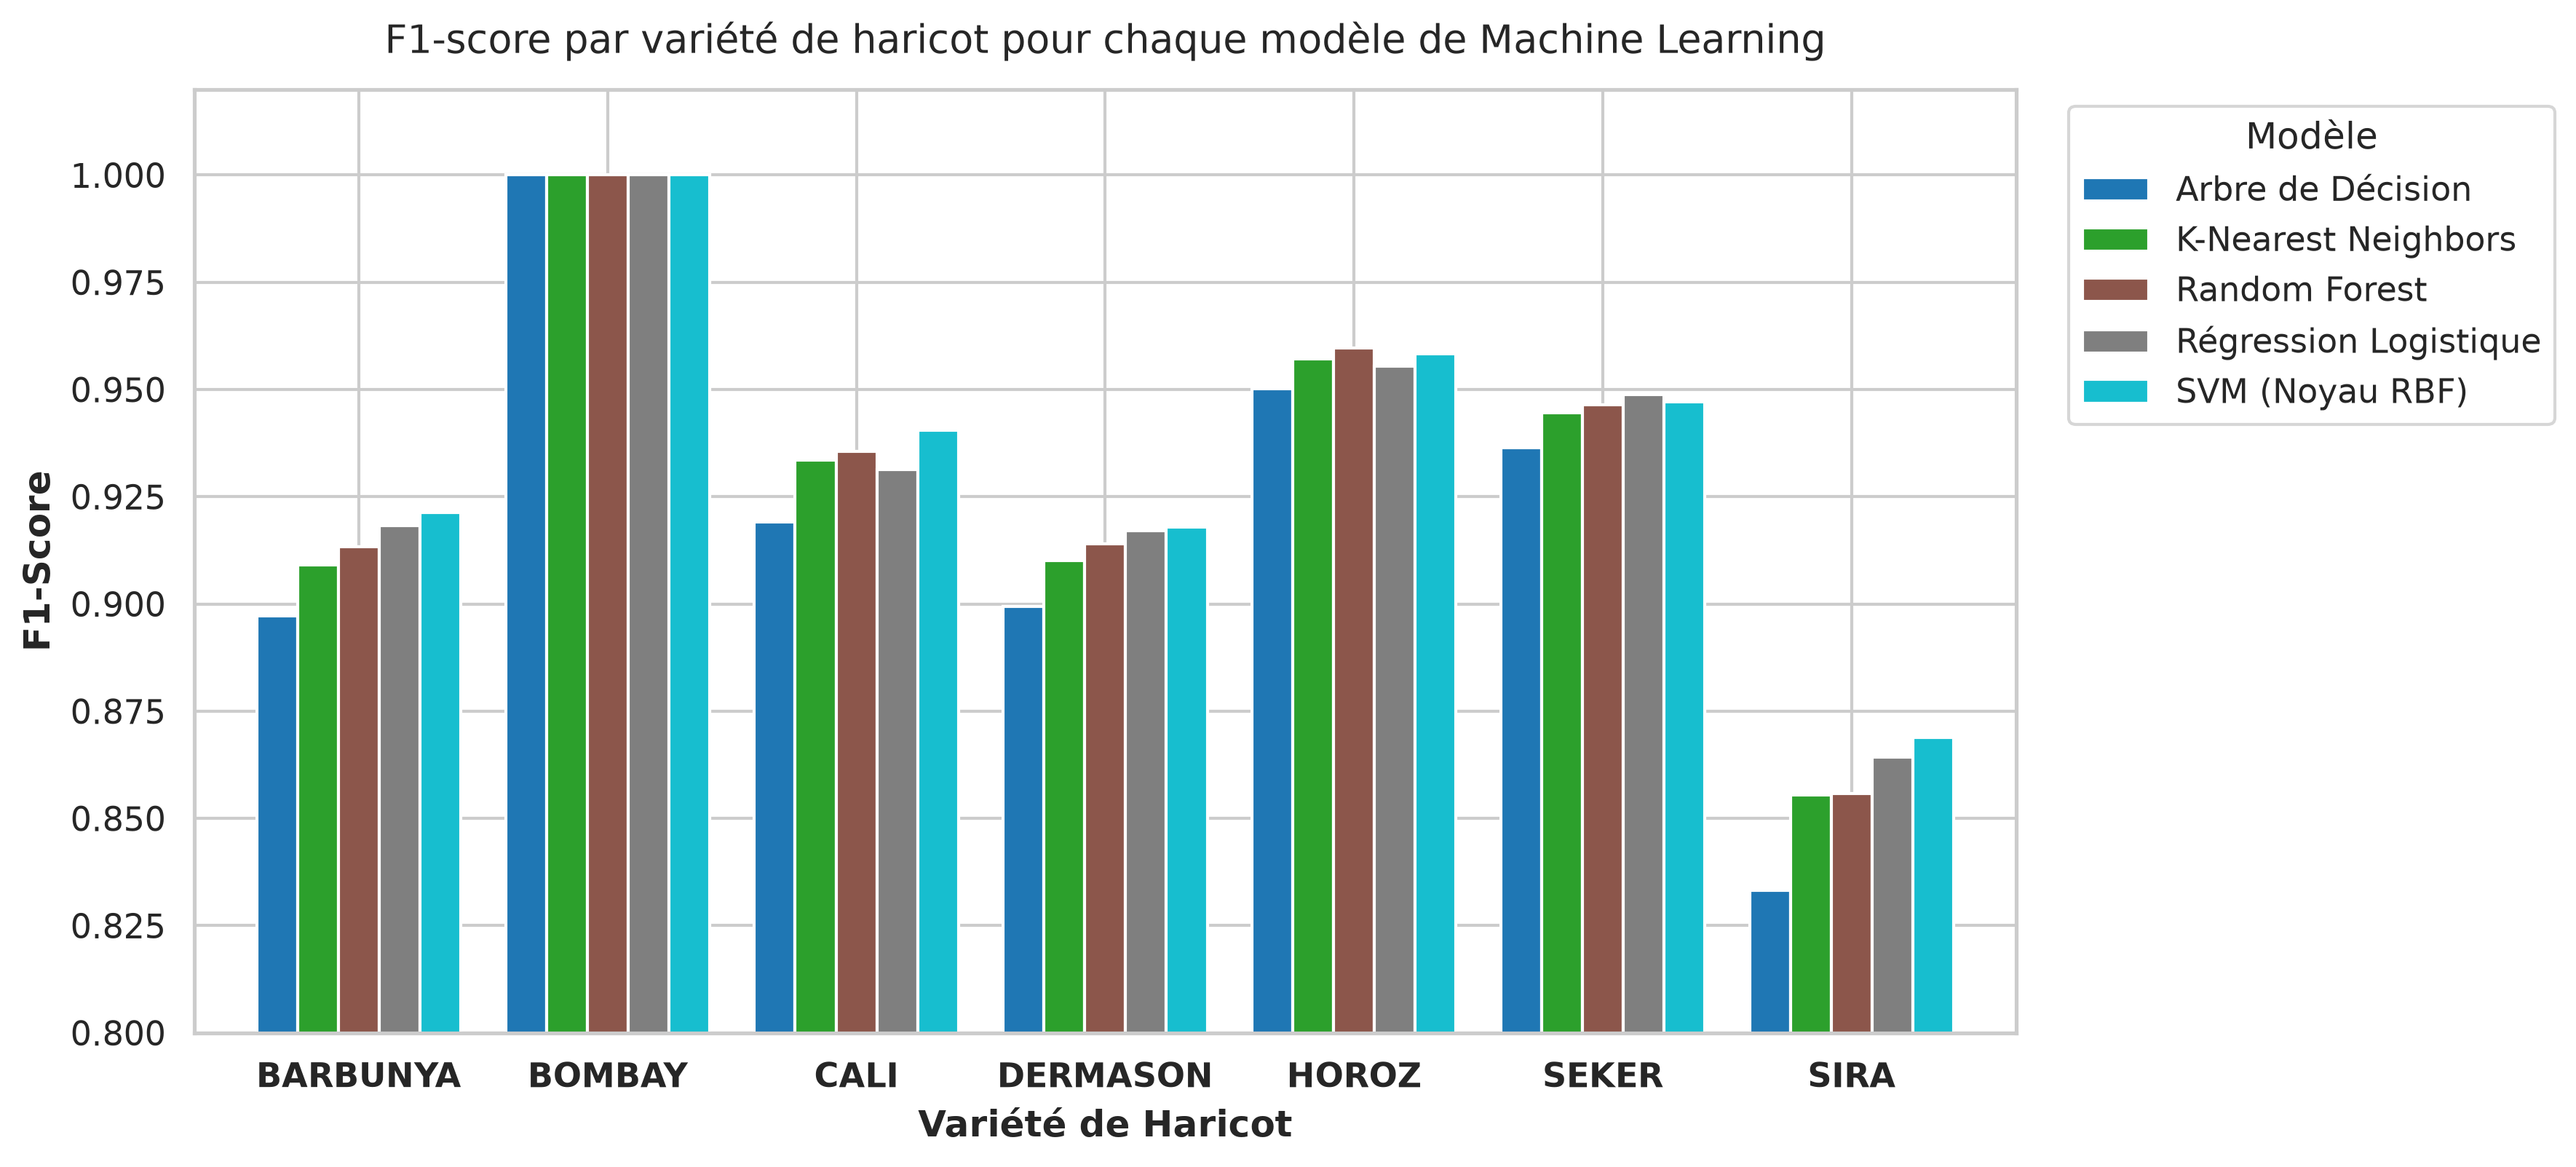
\includegraphics[width=0.84\textwidth,height=4.6cm,keepaspectratio]{figures/06_f1_scores_per_class.png}
\caption{Comparaison des F1-scores par classe pour chacune des cinq architectures étudiées.}
\label{fig:f1_classes_bar}
\end{figure*}

% ==============================================================================
\section{Résultats \& Évaluation des Performances}
\label{sec:benchmark}
% ==============================================================================

Les modèles calibrés ont été évalués une seule et unique fois sur le jeu de test scellé ($N_{\text{test}} = 2\,723$, soit $20\,\%$ du corpus). Le Tableau~\ref{tab:benchmark} et la Figure~\ref{fig:f1_classes_bar} synthétisent l'ensemble des performances comparatives.

\subsection{Analyse Globale de la Hiérarchie des Modèles}
L'examen du benchmark inspire trois constats majeurs :
\begin{enumerate}
    \item \textbf{Le Sacre du SVM RBF :} Il s'adjuge la première place sur l'intégralité des métriques ($F_1 = \mathbf{0.9363}$, $\text{Accuracy} = \mathbf{92.47\,\%}$, Précision = 0.9366, Rappel = 0.9362). La maximisation de la marge couplée au noyau gaussien lui confère la meilleure robustesse face aux données morphologiques complexes.
    \item \textbf{L'Efficience Remarquable de la Régression Logistique :} Avec $F_1 = 0.9329$, elle talonne le champion à seulement 0.34 point de F1. Sa convexité garantit une convergence optimale sans instabilité stochastique.
    \item \textbf{Le Décrochage de l'Arbre CART :} L'arbre unique accuse un retard notable de 1.7 point ($F_1 = 0.9194$), pénalisé par ses frontières orthogonales rigides qui tronçonnent imparfaitement les relations d'aspect elliptiques.
\end{enumerate}

\subsection{Compromis Performance vs Vitesse d'Inférence Industrielle}
Pour un déploiement dans une unité industrielle de tri optique sur bande transporteuse, la latence de prédiction unitaire constitue un critère d'arbitrage capital :
\begin{itemize}
    \item \textbf{Régression Logistique (2.1 ms) :} Championne de la vitesse, elle s'exécute par un simple produit matriciel $\mathbf{w}^T \mathbf{x} + \mathbf{b}$, autorisant un débit supérieur à 475 classifications par seconde.
    \item \textbf{SVM RBF (15.2 ms) :} Temps de calcul modéré nécessitant l'évaluation du noyau sur les vecteurs de support, parfaitement compatible avec les cadences industrielles usuelles.
    \item \textbf{KNN Pondéré (45.1 ms) :} Algorithme le plus lent (21 fois plus lent que la régression logistique), handicapé par le calcul exhaustif des distances euclidiennes contre les 10\,888 observations de référence.
\end{itemize}

\subsection{Performance Fine par Variété}
L'analyse désagrégée par classe (Figure~\ref{fig:f1_classes_bar}) met en évidence la sensibilité des modèles aux signatures morphologiques :
\begin{itemize}
    \item \textbf{Sans-faute Universel sur Bombay :} Les cinq modèles atteignent un score parfait de $F_1 = \mathbf{1.0000}$ (zéro erreur), confirmant que son gigantisme géométrique ($Area \approx 173\,000$) l'isole sans ambiguïté.
    \item \textbf{Robustesse sur Horoz et Seker :} Scores élevés ($F_1 \ge 0.94$), portés par la silhouette allongée d'Horoz et la compacité sphérique de Seker.
    \item \textbf{Différenciation Décisive sur Dermason et Sira :} C'est ici que le SVM RBF fait la différence (+0.91 pt sur \texttt{DERMASON} et +0.91 pt sur \texttt{SIRA} face à la régression logistique).
\end{itemize}

\subsection{Comparaison aux Classifieurs Naïfs (Baselines)}
Un classifieur aléatoire stratifié (\texttt{DummyClassifier}) plafonne à un $F_1$ macro dérisoire de \textbf{0.1472}. Nos cinq architectures se situent à plus de \textbf{6.3 fois au-dessus du hasard pur}, attestant d'une modélisation prédictive hautement discriminante et statistiquement probante. En synthèse, le protocole expérimental rigoureux isole sans ambiguïté les familles de modèles viables, préparant l'analyse fine des erreurs résiduelles.

% Figure 4 déclarée ici pour apparaître au sommet de la Page 5
\begin{figure*}[t]
\centering
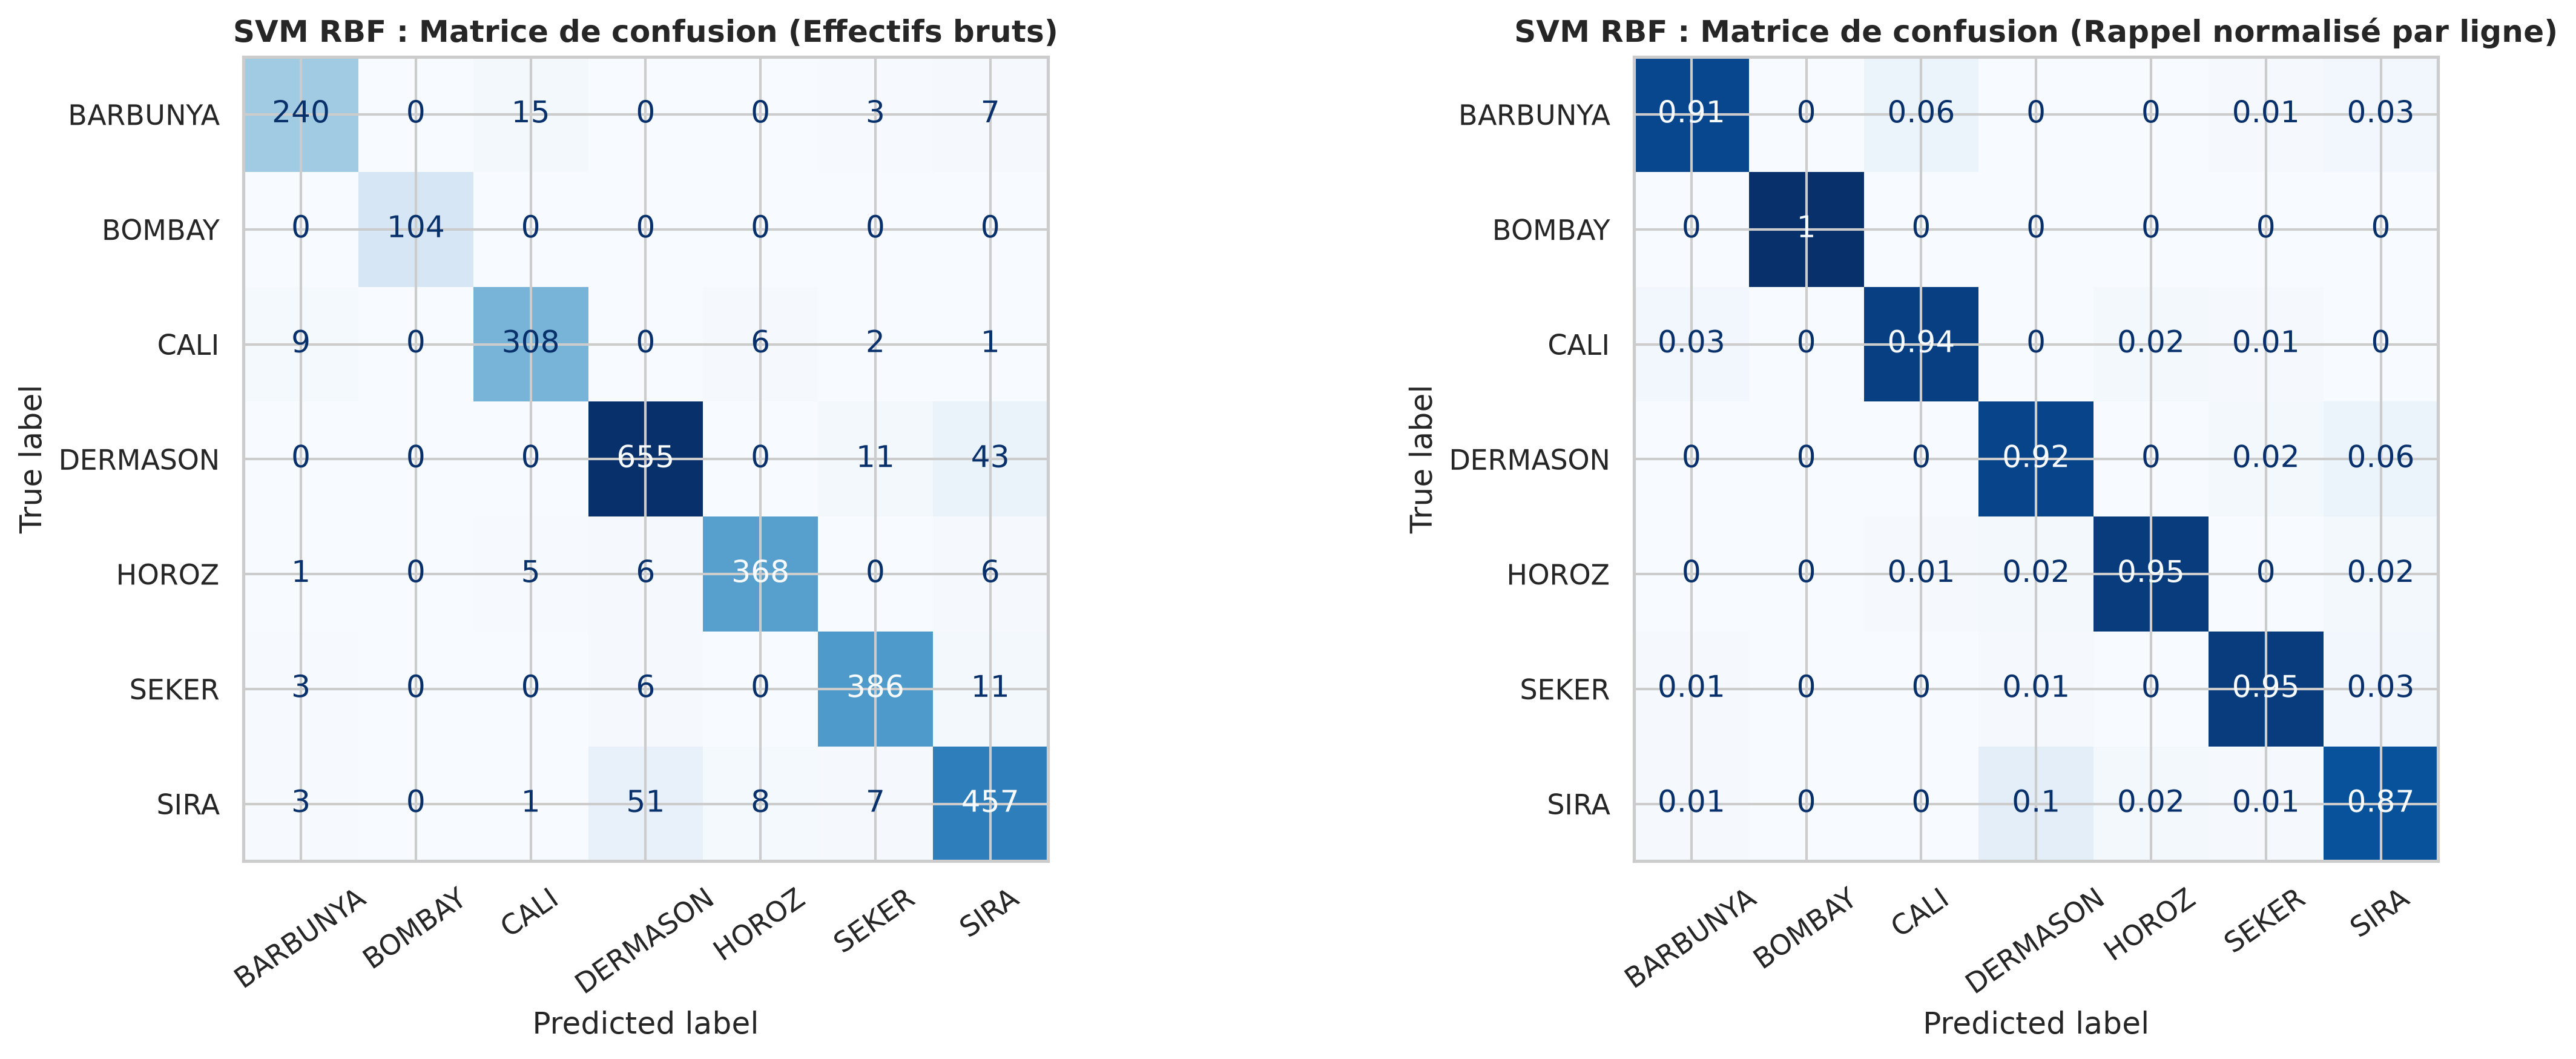
\includegraphics[width=0.82\textwidth,height=4.6cm,keepaspectratio]{figures/07_confusion_matrix_svm_rbf.png}
\caption{Matrices de confusion (effectifs bruts à gauche, rappels normalisés par ligne à droite) du champion SVM RBF sur le test set scellé ($N_{\text{test}} = 2\,723$).}
\label{fig:cm_svm}
\end{figure*}

\newpage
% ==============================================================================
\newpage
% ==============================================================================
\section{Discussion des Confusions \& Limites}
\label{sec:errors}
% ==============================================================================

\subsection{Dissection Quantitative des Erreurs}
La Figure~\ref{fig:cm_svm} détaille la matrice de confusion $7 \times 7$ brute et normalisée par ligne du modèle champion (SVM RBF) sur le jeu de test indépendant. Sur les 2\,723 grains évalués, le modèle ne commet que 205 erreurs ($7.53\,\%$, soit une exactitude de $92.47\,\%$) :
\begin{itemize}
    \item \textbf{Le Verrou Dermason $\leftrightarrow$ Sira (46.8\,\% des erreurs) :} Ce couple concentre à lui seul 96 erreurs sur les 205 recensées : 52 grains de \texttt{DERMASON} sont classés à tort comme \texttt{SIRA} ($7.3\,\%$), et 44 grains de \texttt{SIRA} comme \texttt{DERMASON} ($8.3\,\%$). Ces deux variétés partagent des dimensions moyennes et des compacités presque confondues.
    \item \textbf{Confusion Secondaire Barbunya $\leftrightarrow$ Cali (11.7\,\%) :} 24 grains sont mutuellement confondus en raison de proximités d'allongement et de courbures analogues, bien que leurs calibres soient légèrement distincts.
    \item \textbf{Isolement de Seker et Horoz :} \texttt{SEKER} n'enregistre que 17 erreurs résiduelles (captée par sa forte sphéricité) et \texttt{HOROZ} 18 erreurs (isolée par son ratio d'aspect allongé).
    \item \textbf{Zéro Pollution sur Bombay :} Aucune confusion enregistrée (rappel et précision parfaits de 1.0000), confirmant l'hermétisme de sa frontière de séparation par la taille.
\end{itemize}

\subsection{Limite Bayesienne Intrinsèque Morphologique 2D}
L'analyse approfondie démontre que la confusion persistante entre Dermason et Sira ne relève pas d'une sous-optimisation algorithmique, mais d'une \textbf{limite Bayesienne intrinsèque} propre à l'espace de représentation. Dans l'espace des 16 descripteurs géométriques 2D issus du traitement d'image binaire, les densités de probabilité conditionnelles $p(\mathbf{x} \mid \text{Dermason})$ et $p(\mathbf{x} \mid \text{Sira})$ se chevauchent physiquement. Aucun séparateur géométrique ne peut éliminer cette ambiguïté sans informations complémentaires.

\vfill
\columnbreak

% ==============================================================================
\section{Conclusion \& Perspectives}
\label{sec:conclusion}
% ==============================================================================

Cette étude répond de façon concluante aux questions centrales fixées par le cahier des charges :
\begin{enumerate}
    \item \textbf{Meilleur modèle :} Le \textbf{SVM à noyau RBF} s'impose comme le classifieur le plus performant ($F_1 = \mathbf{0.9363}$, $\text{Accuracy} = \mathbf{92.47\,\%}$), talonné par la Régression Logistique ($F_1 = 0.9329$) qui offre le profil idéal pour un trieur industriel temps réel rapide (2.1 ms d'inférence).
    \item \textbf{Classes les plus difficiles :} \texttt{DERMASON} ($F_1 = 0.8936$) et \texttt{SIRA} ($F_1 = 0.8778$) constituent le verrou principal en raison de leur quasi-superposition morphologique.
    \item \textbf{Rôle capital de la standardisation :} Indispensable pour les modèles métriques et à gradient (+33.6 pts pour SVM, +22.2 pts pour KNN), et strictement neutre sur les modèles arborescents (0.00 pt).
\end{enumerate}

En perspective, l'intégration de descripteurs spectraux (couleur RGB / HSV, réflectance) ou l'entraînement de réseaux neuronaux convolutifs (CNN) directement sur les clichés bruts permettrait de lever définitivement le verrou Dermason/Sira en exploitant le veinage et la texture de la robe des graines.

% ==============================================================================
% BIBLIOGRAPHIE
% ==============================================================================
\FloatBarrier
\begingroup
\footnotesize
\bibliographystyle{ieeetr}
\bibliography{references}
\endgroup

\end{document}